\documentclass[tikz,border=2pt]{standalone}
\renewcommand{\familydefault}{\sfdefault}
\usetikzlibrary{arrows.meta,calc,positioning}
\tikzset{every picture/.style={line width=1pt, >=Stealth},
         hl/.style={fill=black, fill opacity=0.12, text opacity=1}}
\begin{document}
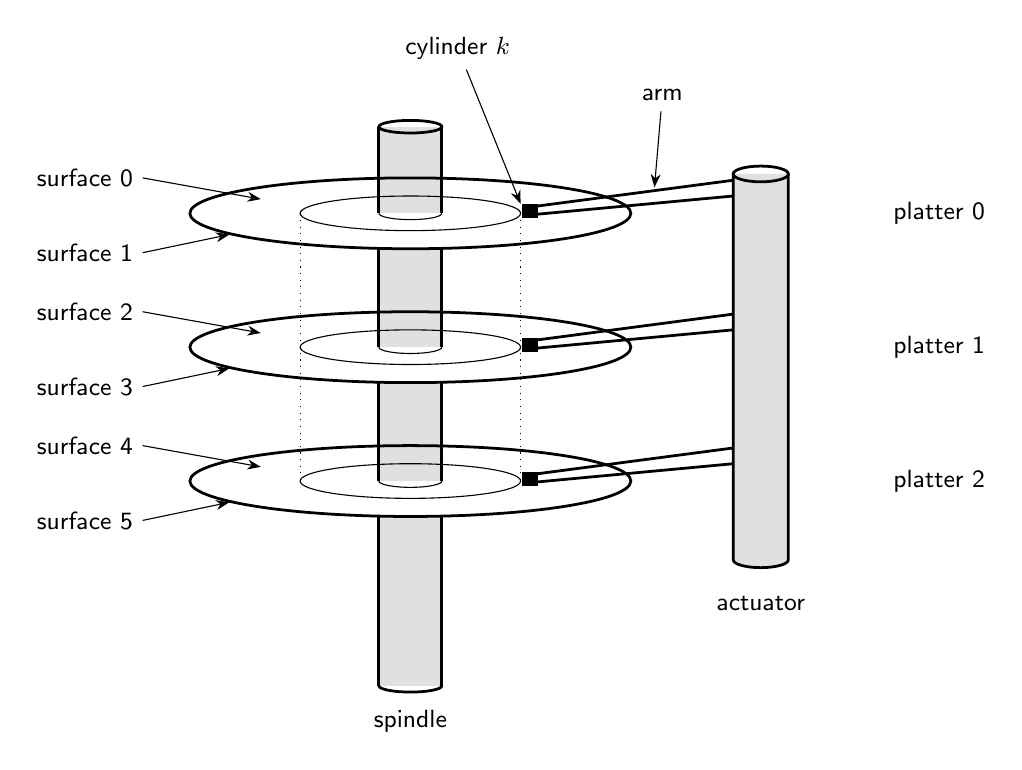
\begin{tikzpicture}[note/.style={font=\small}]
  % Three platters on one spindle, seen from slightly above. Platter i sits at height -1.7i.
  \def\R{2.8}\def\r{0.45}\def\k{1.4}
  % Spindle: only the parts not hidden behind a platter (each platter's front edge is \r below its centre).
  \foreach \lo/\hi in {0/1.1, -1.7/-0.45, -3.4/-2.15, -6/-3.85} {
    \fill[black, fill opacity=0.12] (-0.4, \lo) rectangle (0.4, \hi);
    \draw (-0.4, \lo) -- (-0.4, \hi) (0.4, \lo) -- (0.4, \hi);
  }
  \draw (0, 1.1) ellipse (0.4 and 0.08);
  \draw (-0.4, -6) arc[start angle=180, end angle=360, x radius=0.4, y radius=0.08];
  \foreach \y in {0, -1.7, -3.4} \draw[thin] (-0.4, \y) arc[start angle=180, end angle=360, x radius=0.4, y radius=0.08];
  % Platters, each with the track that belongs to cylinder k.
  \foreach \i in {0, 1, 2} {
    \pgfmathsetmacro{\y}{-1.7*\i}
    \draw (0, \y) ellipse (\R cm and \r cm);
    \draw[thin] (0, \y) ellipse (\k cm and 0.22cm);
    \node[note, anchor=west] at (6, \y) {platter \i};
  }
  \foreach \x in {-\k, \k} \draw[thin, dotted] (\x, 0) -- (\x, -3.4);
  % Surfaces: the upper and lower side of each platter.
  \foreach \i in {0, 1, 2} {
    \pgfmathsetmacro{\y}{-1.7*\i}
    \pgfmathtruncatemacro{\up}{2*\i}\pgfmathtruncatemacro{\down}{2*\i + 1}
    \draw[<-, thin] (-1.9, \y + 0.18) -- (-3.4, \y + 0.45) node[left, note] {surface \up};
    \draw[<-, thin] (-2.3, \y - 0.27) -- (-3.4, \y - 0.5) node[left, note] {surface \down};
  }
  % Actuator: one column whose arms move every read/write head together.
  \draw[hl] (4.1, 0.5) -- (4.1, -4.4) arc[start angle=180, end angle=360, x radius=0.35, y radius=0.1] -- (4.8, 0.5);
  \draw (4.45, 0.5) ellipse (0.35 and 0.1);
  \foreach \i in {0, 1, 2} {
    \pgfmathsetmacro{\y}{-1.7*\i}
    \draw (4.1, \y + 0.42) -- (\k + 0.12, \y + 0.08) -- (\k + 0.12, \y - 0.02) -- (4.1, \y + 0.22);
    \fill (\k + 0.02, \y - 0.06) rectangle (\k + 0.22, \y + 0.12);
  }
  \node[note] (cyl) at (0.6, 2.1) {cylinder $k$};
  \draw[->, thin] (cyl) -- (\k, 0.12);
  \node[note] (arm) at (3.2, 1.5) {arm};
  \draw[->, thin] (arm) -- (3.1, 0.33);
  \node[note] at (4.45, -4.95) {actuator};
  \node[note] at (0, -6.45) {spindle};
\end{tikzpicture}
\end{document}
